\documentclass[11pt]{article}
\usepackage[utf8]{inputenc}
\usepackage[T1]{fontenc}
\usepackage{graphicx} % Required for inserting images
\usepackage{amsmath} % For \text and math environments
\usepackage{geometry} % For margin settings
\usepackage{hyperref} % For clickable links
\usepackage[backend=biber, style=authoryear]{biblatex}
\usepackage{float}

\geometry{margin=1in}
\addbibresource{references.bib}

\title{\textbf{Optimizing Autonomous Fleet Logistics via Proximal Policy Optimization}}
\author{Aksel Kretsinger-Walters, Alena Chan, Andrey Aksyutkin}
\date{December 2025}

\begin{document}

\maketitle

\begin{abstract}
		This report details the application of Reinforcement Learning (RL) to the complex logistics of autonomous
		robotaxi fleets. We model the city environment as a dynamic graph and utilize Proximal Policy Optimization
		(PPO) to maximize fleet profitability and demand satisfaction. By encoding the city as a network of
		connected nodes—representing vehicle availability and demand hotspots—we demonstrate that PPO with clipped
		updates generates stable and profitable policies compared to baseline heuristics. We further analyze the
		impact of high-reward "red nodes" and their adjacent "orange nodes" on agent behavior within our simulation.
\end{abstract}

\section{Introduction}

One of the most promising and revolutionary applications of reinforcement learning (RL) is in the domain of
autonomous logistics, specifically self-driving car fleets. The challenges facing the autonomous vehicle
community span multiple dimensions, including intellectual, ethical, financial, and technical hurdles. In
this project, we narrow our focus to optimizing the operational profitability of robo-taxi fleets.

The relevance of this domain is underscored by its enormous commercial and consumer potential. Commercially,
applications extend to freight, last-mile delivery, and industrial logistics. On the consumer side, the
technology enables robotaxis, improved public transportation, and critical response systems that enhance
safety and accessibility. Effectively managing such fleets solves key problems in inventory management and
urban planning.

However, monitoring, maintaining, and optimizing a large fleet of self-driving cars is a non-trivial problem.
Operators must maximize availability, minimize downtime, and ensure network resilience. Furthermore, they
must accurately predict supply and demand to facilitate dynamic pricing and maximize utilization efficiency.
While tasks such as scheduling maintenance, recharging vehicles, and minimizing wait times are difficult
individually, jointly optimizing across all these dimensions while adapting to distribution shifts is
significantly more challenging. This interactive, multi-objective nature makes the problem a natural
candidate for reinforcement learning and agentic approaches.

\section{Methodology}

% \subsection{RL Formulation}
% We simulate a fleet of self-driving cars as a Markov Decision Process (MDP) to develop algorithms that
% optimize operations and profitability.
% \begin{itemize}
% 		\item \textbf{State Space:} The state includes the location of each car, the distribution of passenger
% 				demand, and current weather conditions. We include weather as it has been shown that meteorological
% 				factors significantly drive the location and volume of demand, accounting for substantial variance in
% 				ride-hailing profits.
% 		\item \textbf{Action Space:} The action space consists of directing each car to move in one of the cardinal
% 				directions (North, South, East, West) or stay put.
% \end{itemize}

% While the problem could be approached by having each car make location decisions independently, implicit
% coordination often makes such solutions unstable. Therefore, we utilize a centralized policy approach.

\subsection{Environment and Simulation}
\label{sec:env}

We modeled the city as a graph of nodes representing pickup and drop-off locations, with edges representing
the roads connecting them. Leveraging the regular structure of cities like New York, we utilized a grid
representation where road distances are estimated using Manhattan distance. To limit training time—since the
state-action space scales linearly with grid size—we initially evaluated basic policies on a simplified $4
\times 5$ graph before scaling to larger simulations.

\paragraph{Gymnasium Framework}
We built our simulation environment using the OpenAI Gymnasium scaffolding. Gymnasium abstracts away
many implementation details, allowing us to focus on defining the state space, action space, transition
model, and reward structures as follows.

\paragraph{OSMnx Integration} For the Manhattan simulation, we utilized OSMnx to extract a realistic road network
graph from OpenStreetMap data. This allowed us to model the city's irregular layout and road connectivity
accurately, providing a more challenging and realistic environment for our RL agent.

\paragraph{State Space} The state space was deliberately abstracted away from the underlying graph. This
decision was made to facilitate generalization to unseen cities with different layouts. The state provided to
the agent included:
% \begin{itemize}
% 		\item \textbf{Globals (Vector)} Time of day (normalized to the unit circle), Day of week (normalized to
% the unit circle), Weather state (categorical variable representing weather conditions).
% 		\item \textbf{Supply-Demand Conditions (Vector)} The current ratio of available cars to ride requests
% awaiting dispatch (requests that had accepted the price provided to them from the model in the step prior)
% \end{itemize}

\begin{itemize}
		\item \textbf{Globals (Vector)} These global context variables provide the model with temporal and
				environmental information, allowing it to learn the latent patterns in demand fluctuations
				\begin{enumerate}
						\item Time of day (normalized to the unit circle)
						\item Day of week (normalized to the unit circle)
						\item Weather state (categorical variable representing weather conditions)
				\end{enumerate}
		\item \textbf{Supply-Demand Conditions (Vector)} These variables inform the agent about the current state
				of supply and demand in the environment
				\begin{enumerate}
						\item The current ratio of available cars to ride requests awaiting dispatch (requests that had
								accepted the price provided to them from the model in the step prior)
						\item Vehicles per nodes
						\item Mean lambda value per node (sampled each step from a Poisson distribution with parameter $\lambda$)
				\end{enumerate}
		\item \textbf{Vehicles (Matrix)} A matrix representation of the vehicles in the environment
				\begin{enumerate}
						\item Location (X coordinate) - Normalized to [-1, 1]
						\item Location (Y coordinate) - Normalized to [-1, 1]
						\item Battery level - Normalized to [0, 1]
						\item Status: {Idle, Assigned, In-Transit, Charging} - One-hot encoded
				\end{enumerate}
		\item \textbf{Pending Requests (Matrix)} A matrix representation of the pending requests in the environment
				\begin{enumerate}
						\item Pickup Location (X coordinate) - Normalized to [-1, 1]
						\item Pickup Location (Y coordinate) - Normalized to [-1, 1]
						\item Drop-off Location (X coordinate) - Normalized to [-1, 1]
						\item Drop-off Location (Y coordinate) - Normalized to [-1, 1]
						\item Cust bias (coefficient representing customers' base willingness to pay)
						\item Cust temperature (coefficient representing customers' sensitivity to price changes)
						\item Estimated Cost (linear product of distance and a per-unit distance cost)
						\item Max Wait Time (in time steps) - Maximum time a customer is willing to wait for pickup once
								they've accepted the price
						\item Wait Time (in time steps) - Current time the customer has been waiting for pickup
						\item Status: {Expired, Price Rejected, Awaiting Price, Accepted Price (awaiting pickup), Assigned
								(vehicle en route), In-Transit} - One-hot encoded
				\end{enumerate}
		\item \textbf{Active Rides (Matrix)}
				\begin{enumerate}
						\item Pickups \& Drop off location, Estimated Cost - (duplicated from matched request)
						\item Price - Price agreed
						\item Total Distance - Total distance of the ride
						\item Distance Traveled - Distance traveled so far
				\end{enumerate}
		\item \textbf{Dispatch Mask (Vector)} A binary vector indicating which vehicles are eligible for
				dispatching to new requests (1 if eligible, 0 otherwise)
		\item \textbf{Pricing Mask (Vector)} A binary vector indicating which requests are eligible for pricing (1
				if eligible, 0 otherwise)
\end{itemize}

\paragraph{Action Space} The actions available to the agent at each time step included
\begin{itemize}
		\item \textbf{Prices:} For each pending request, the price to offer the customer
		\item \textbf{Repositioning:} For each vehicle, the desired (x, y) location to move towards
		\item \textbf{Dispatch Decisions:} For each request, a one-hot encoded vector indicating which vehicle to
				dispatch (or none)
\end{itemize}
\paragraph{Transition Model} The environment's transition dynamics were modeled to reflect realistic
interactions:
\begin{itemize}
		\item \textbf{Action Application:}
				\begin{enumerate}
						\item \textbf{Pricing Action:} Calculate the z-score of the probability of acceptance based on price,
								supply demand imbalance, weather, estimated cost, cusomter bias \& temperature.
						\item \textbf{Reposition Action:} Move \textbf{idle} vehicles towards their target locations.
						\item \textbf{Dispatch Action:} Assign vehicles to requests based on the dispatch decisions made by the agent.
				\end{enumerate}
		\item \textbf{State Management:}
				\begin{enumerate}
						\item \textbf{Spawn New Requests:} New ride requests were generated based on a Poisson process. Each
								node in the graph has an associated $\lambda$ parameter, dictating the average rate of request
								arrivals. This parameter could vary over time to simulate demand fluctuations.
						\item \textbf{Update Existing Requests:} The wait time for each pending request was incremented;
								requests that exceeded their maximum wait time were marked as expired and removed from the pending list.
						\item \textbf{Update Rides:} Move active rides towards drop-off locations (deterministic, Djikstra);
								complete rides when the destination is reached, freeing up vehicles. Match vehicles to requests upon dispatch.
								% \item \textbf{Update Vehicle Status:} Update the status of each vehicle based on its current
								% activity (e.g., idle, assigned, in-transit, charging).
						\item \textbf{Global Variables}: Update time of day, day of week, and weather conditions as per the
								simulation clock.
				\end{enumerate}
\end{itemize}

\paragraph{Reward Structure} The reward system was designed to allow finetuning, and eventual sparsification of rewards:
\begin{itemize}
		\item \textbf{Dispatches}:
				\begin{itemize}
						\item Penalties: Multiple dispatches to the same vehicle, dispatching an unavailable vehicle, distance
								from vehicle to pickup location (euclidean distance for simplification)
						\item Rewards: None (implicit reward through successful pickups)
				\end{itemize}
		\item \textbf{Requests}:
				\begin{itemize}
						\item Penalties: Expired requests, rejected prices
						\item Rewards: None (implicit reward through successful pickups)
				\end{itemize}
		\item \textbf{Rides}:
				\begin{itemize}
						\item Penalties: cost per km traveled (fuel, time)
						\item Rewards: fare collected per meter traveled, extra reward upon completion
				\end{itemize}
\end{itemize}
% \paragraph{Observation Space and Node Modeling}–
% A key contribution of our environment design is the specific modeling of the city graph provided to the PPO agent:
% \begin{itemize}
%     \item \textbf{Node Representation:} The city is modeled as a set of connected nodes. Crucially, the
% numerical value assigned to each node in the state representation corresponds to the \textbf{number of cars
% available} at that node at the current moment.
%     \item \textbf{Demand Hotspots (Red and Orange Nodes):} To simulate realistic demand spikes, we
% introduced specific node types.
%     \begin{itemize}
%         \item \textbf{Red Nodes:} These represent high-reward, high-payoff, and high-demand points (e.g., a
% stadium after a game or a transit hub).
%         \item \textbf{Orange Nodes:} These nodes are defined as always being adjacent to Red nodes.
%     \end{itemize}
% \end{itemize}
% This topological and demand-specific information—car counts per node and the location of high-value
% Red/Orange nodes—was explicitly provided to the PPO agent during training, allowing it to learn
% anticipation strategies for high-demand events.

\subsection{Proximal Policy Optimization (PPO)}
For the fleet distribution algorithm, we utilize Proximal Policy Optimization (PPO)
\parencite{schulman2017proximal}. PPO is a variation of the actor-critic architecture that updates the policy
using a clipped surrogate objective, denoted as $L_t(\theta)$. This clipping is vital for real-time business
decisions, as it prevents large, destabilizing updates that could, for example, erroneously direct the entire
fleet to a low-demand area.

Stable updates are achieved by maintaining "old" and "current" policy distributions over the state-action
space and limiting the divergence between them. The objective function we maximize via gradient ascent is:
\[
		L_t(\theta) = \min \Big( r_t(\theta)\,\hat{A}_t,\; \text{clip}\big(r_t(\theta),\, 1 - \epsilon,\, 1 +
		\epsilon\big)\,\hat{A}_t \Big)
\]
where $\epsilon$ bounds the divergence (typically $\epsilon \in [0.1, 0.3]$), $r_t(\theta)$ is the
probability ratio of the action under the current vs. old policy, and $\hat{A}_t$ is the estimated advantage.
We found $\epsilon=0.2$ provided the most stable and accurate policy.

Our policy model is a 2-layer neural network with a hidden size of 128 and ReLU activation, optimized using
Adam. The critic (Value Function) shares this architecture but outputs a single value (advantage), optimized
via mean squared error.

\section{Results}

We compared different policies on a 20-node city grid before scaling up to Manhattan (graph sparsified to 782
nodes, from 4k+).
\paragraph{20-node results}
To test robustness, we simulated a high-demand center (controlled by parameter $\lambda$) moving in a
circular trajectory around the city, the position of which was predictable via the weather state provided to
the agent. This assumption is realistic, as autonomous fleets (e.g., Waymo) have access to real-time weather
and event forecasting.

Evaluations were conducted over 20-minute episodes, reflecting the average ride time and the threshold at
which customers typically cancel if a vehicle has not arrived.

\paragraph{Manhattan results}
After validating our approach on the 20-node grid, we scaled our environment to a realistic Manhattan layout.
The complexity of the environment increased significantly, as did the action and observation space. We
weren't able to achieve measurable improvements over our heuristic agent baselines.

\subsection{Policy Gradient vs. Baseline}
\paragraph{20-node Baseline Comparison}
As a baseline, we used a \textbf{NEAREST} car assignment heuristic, where the closest available car is
dispatched to a request. If no demand exists, spare cars move randomly.

We observed that the Policy Gradient approach, which proactively relocates cars and intelligently passes on
suboptimal immediate demand for greater long-term rewards, significantly outperformed the baseline.
\begin{itemize}
		\item \textbf{NEAREST Baseline Profit:} 7,990.71 units
		\item \textbf{Policy Gradient Profit:} 12,829.93 units
		\item \textbf{Improvement:} $\approx 60\%$
\end{itemize}

\begin{figure}[h!]
		\centering
		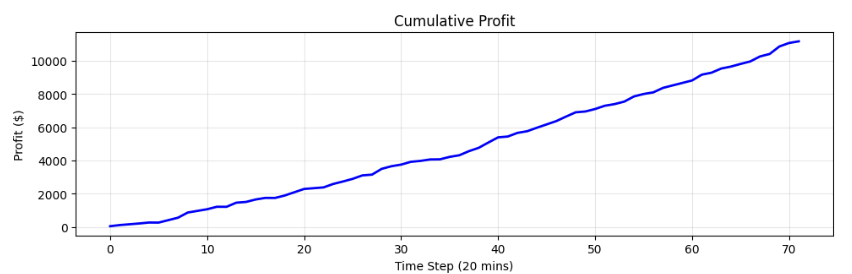
\includegraphics[width=\linewidth]{images/cum-profit-vpg.png}
		\caption{Cumulative profit over a 20-minute episode comparing Policy Gradient to Baseline.}
		\label{fig:profit}
\end{figure}

\paragraph{Manhattan Baseline Comparison}
For the Manhattan environment, we defined the heuristic agents as follows:
\begin{itemize}
		\item \textbf{Pricing Agent:} $\text{Price} = (2 \cdot \text{Estimated Cost}) - \text{Supply/Demand
				Imbalance}$ (Normalized to [0, 1], higher value indicates oversupply)
		\item \textbf{Dispatch Agent:} Iterate through requests, calculate closest vehicle, dispatch if within
				threshold distance; otherwise skip.
		\item \textbf{Repositioning Agent:} Assign vehicles to nodes proportionally to the node's degree centrality
				in the graph.
\end{itemize}

\textbf{TODO - explanation? Figures? debugging? next steps?}
\subsection{Policy Gradient vs. PPO (Clipped)}
We further compared vanilla Vanilla Policy Gradient (VPG) against PPO with clipped updates on the 20-node
grid with circular demand movement.

While PPO with clipping requires longer training times (more iterations) to learn because it bounds
aggressive policy updates, it ultimately achieves higher cumulative rewards and improved stability. This
stability is crucial for complex environments where VPG might collapse into suboptimal deterministic
policies. Our observations align with theoretical findings in \cite{wang2025improving}, which suggest similar
long-term performance between clipped PPO and repeated VPG, though PPO offers safety guarantees essential for
physical deployment.

\begin{figure}[H]
		\centering
		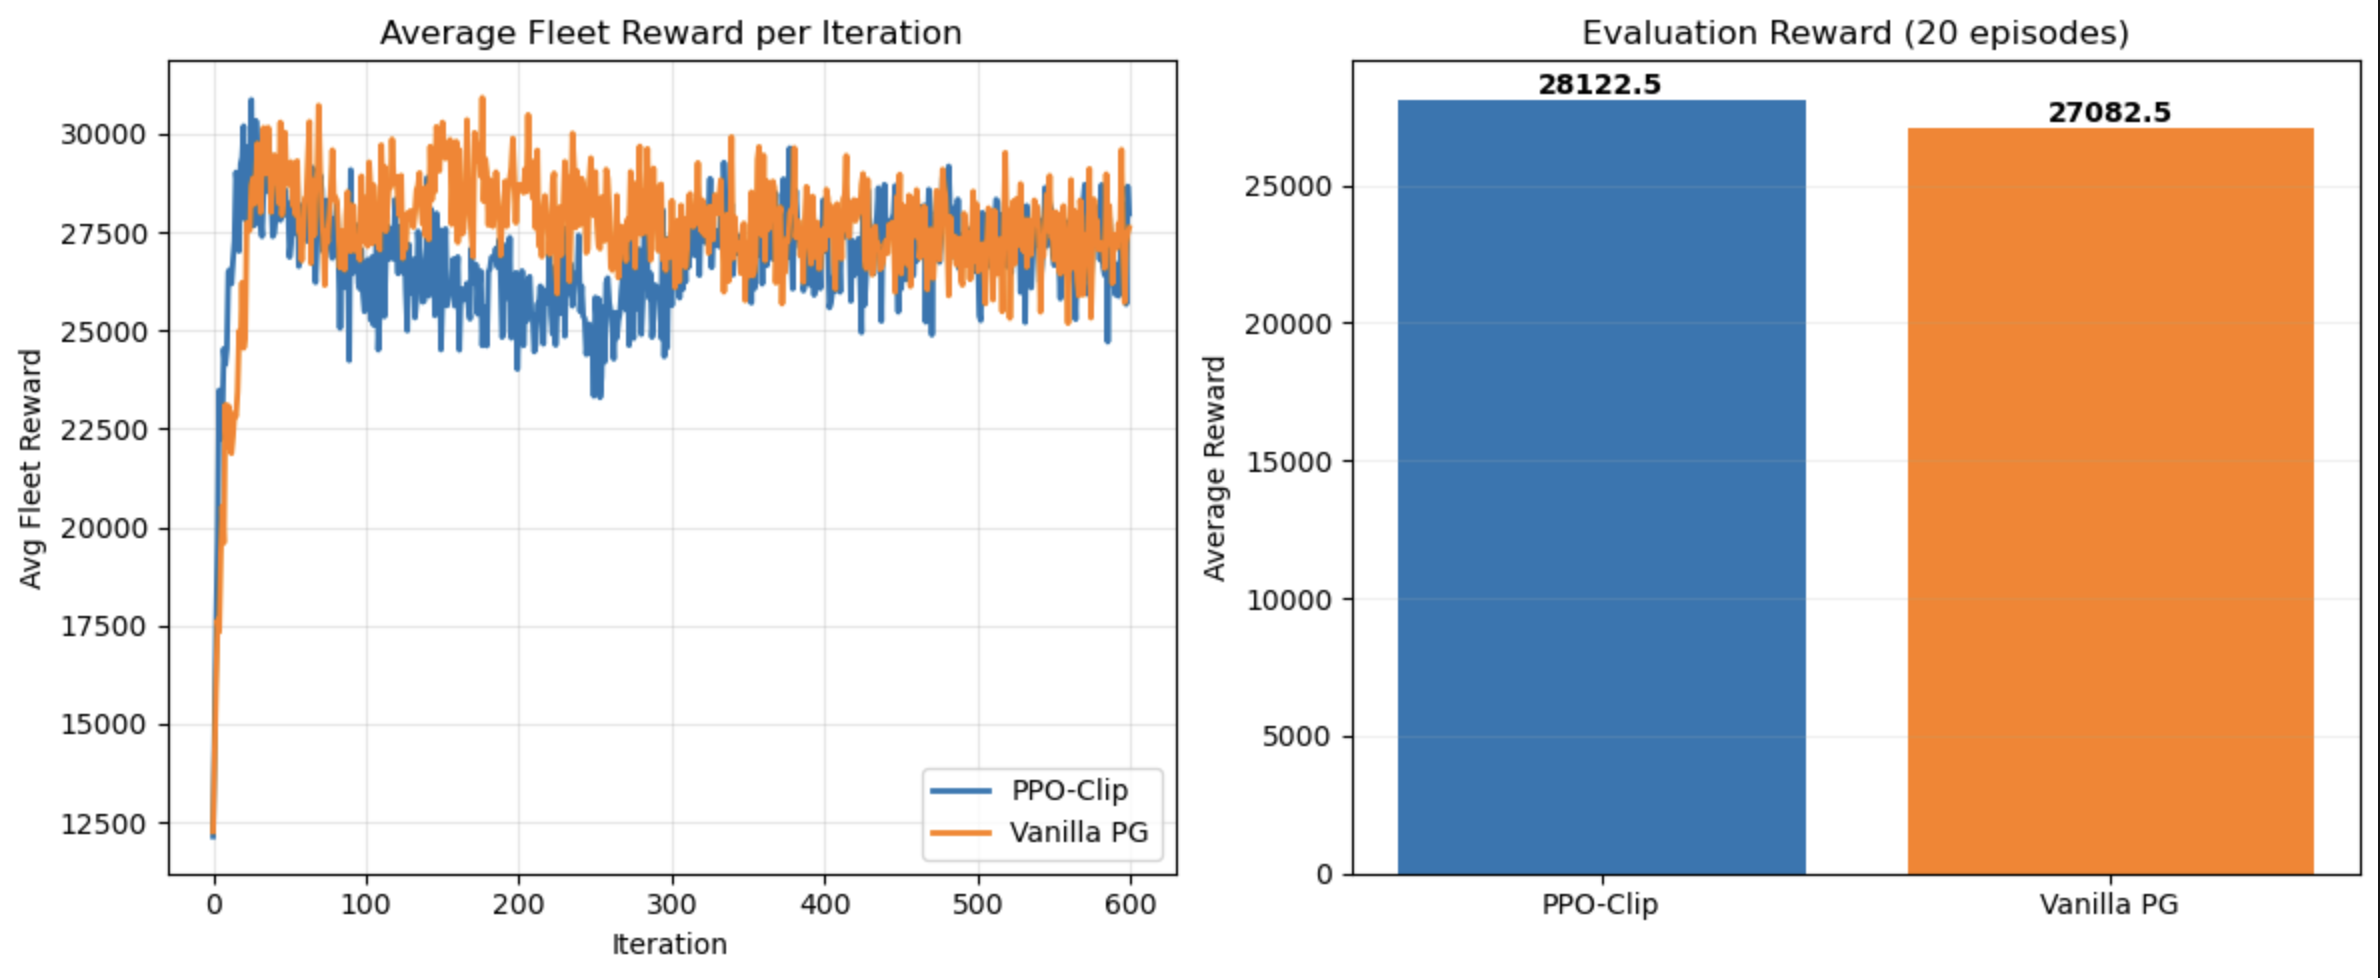
\includegraphics[width=\linewidth]{images/gradinet-vs-ppo.png}
		\caption{Training curves: Gradient policy update vs. PPO with clipping.}
		\label{fig:ppo_comparison}
\end{figure}

\begin{figure}[H]
		\centering
		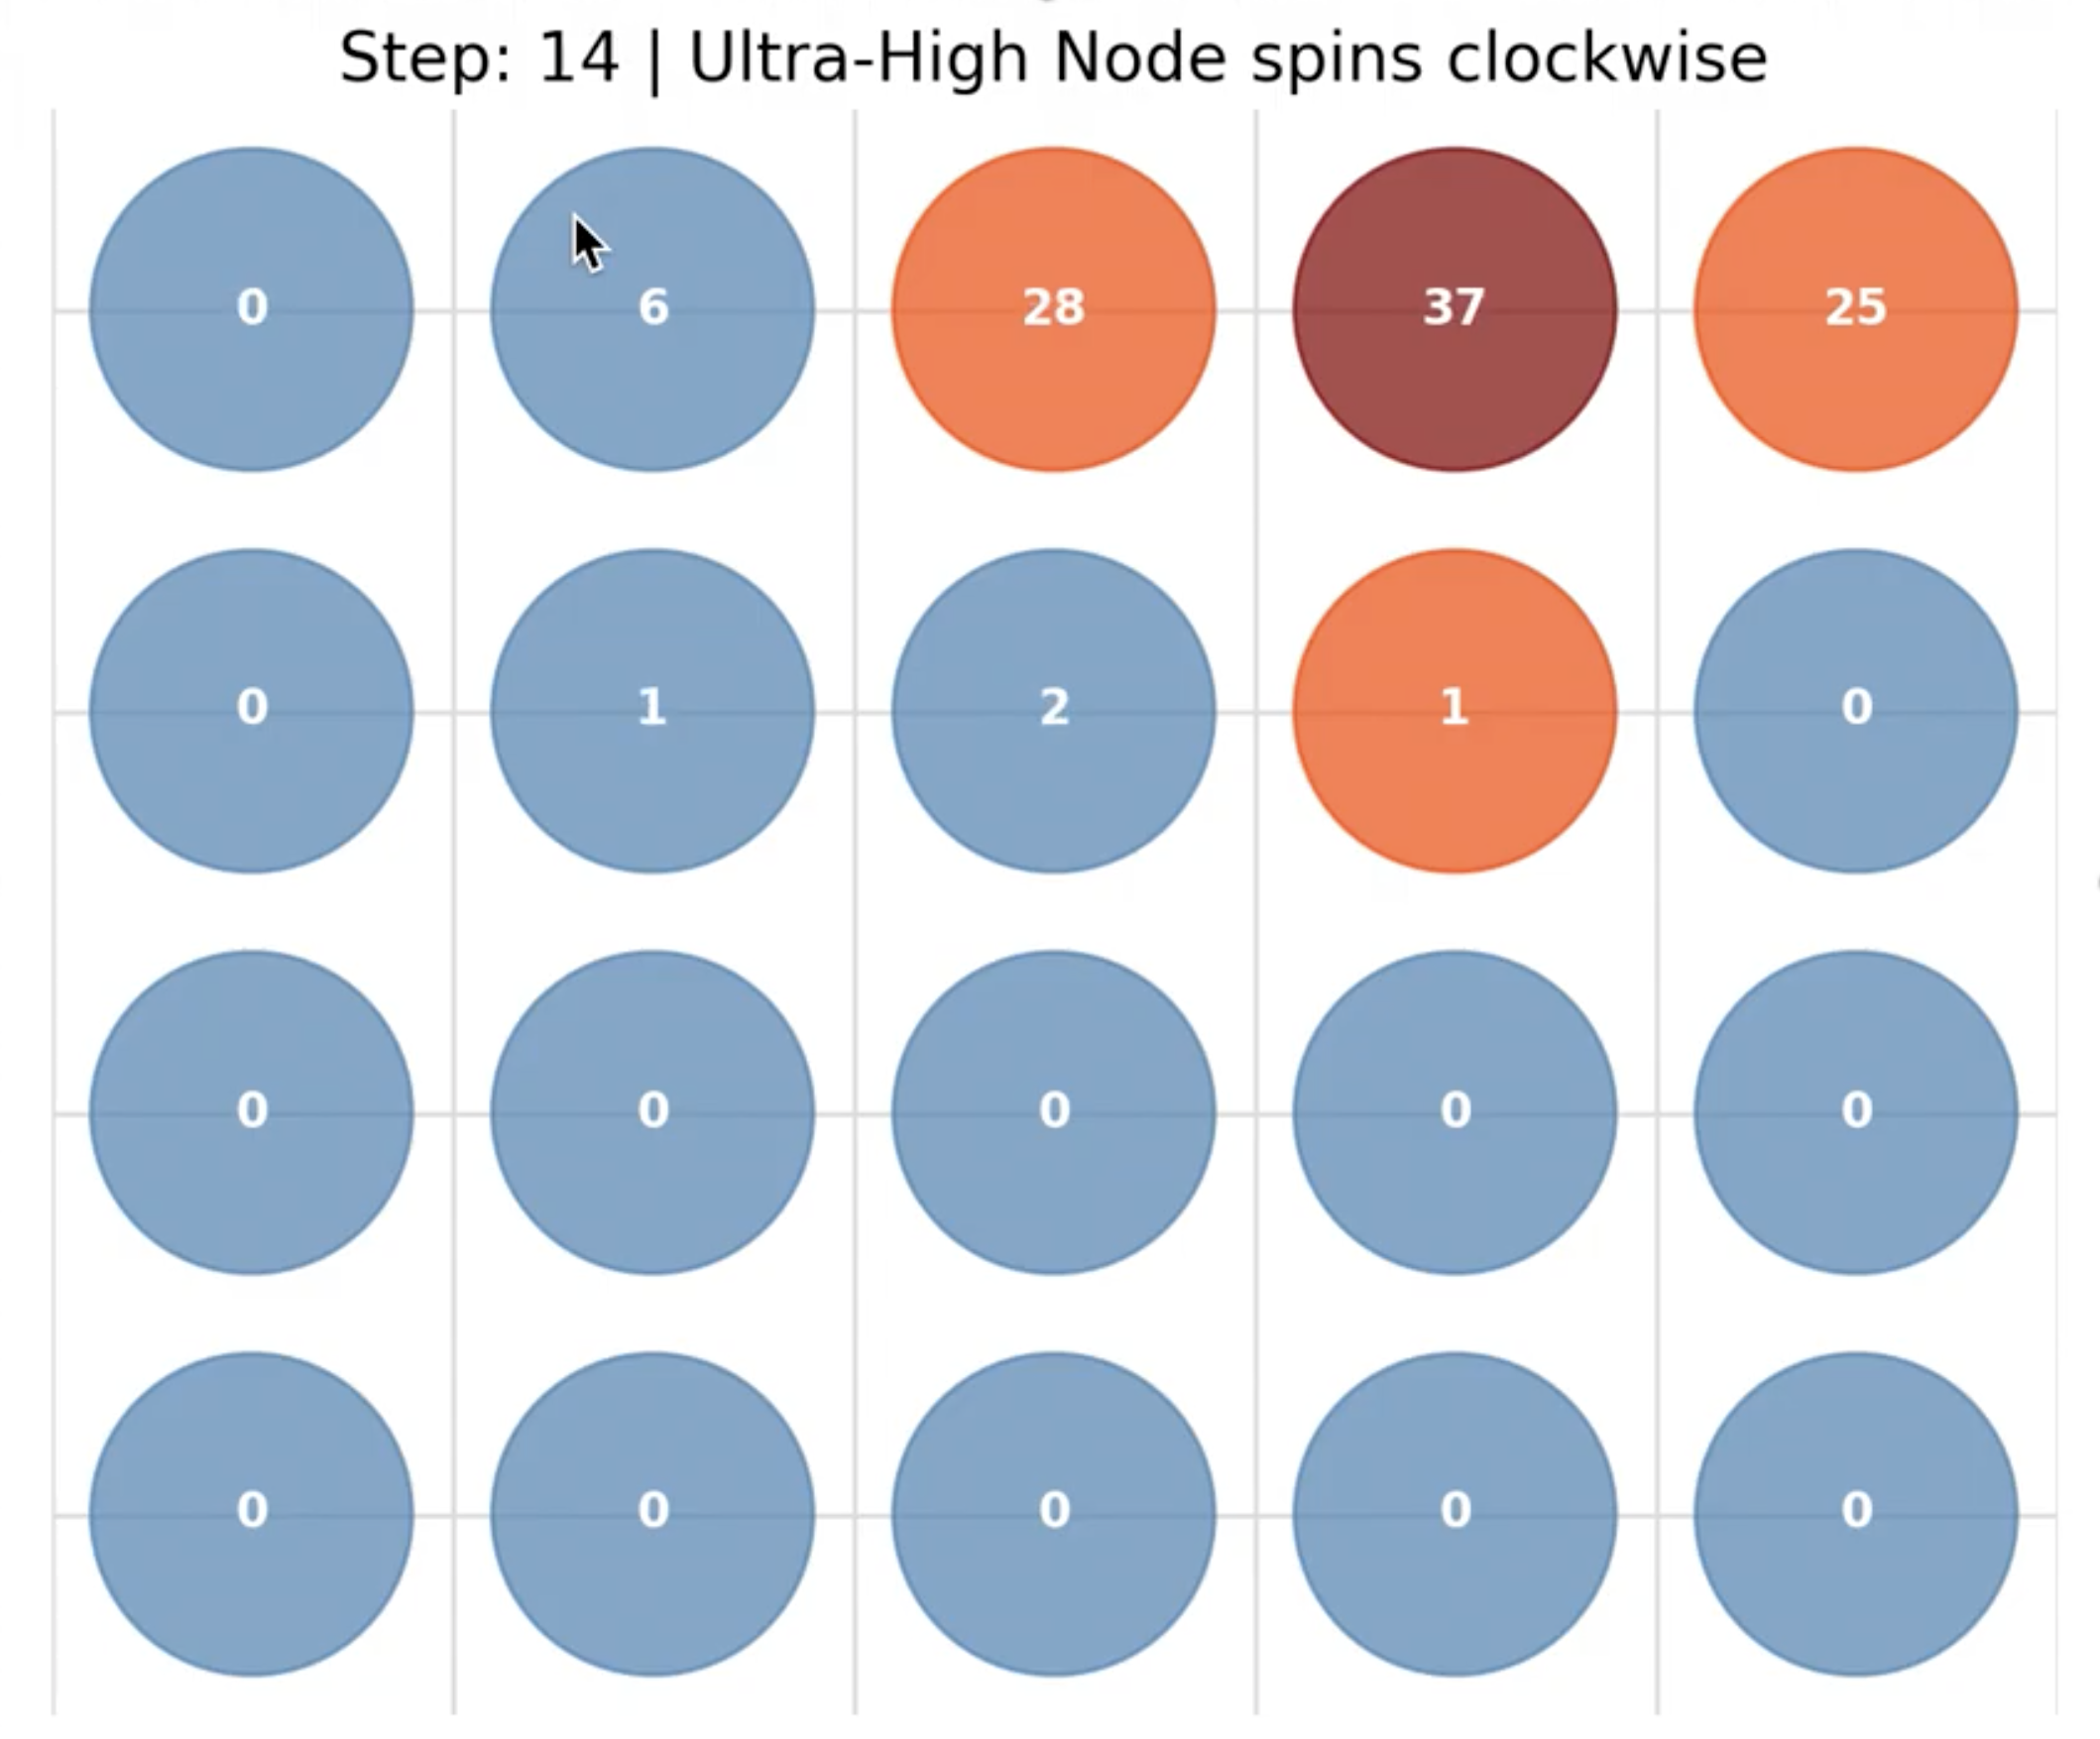
\includegraphics[width=\linewidth]{images/nodes.png}
		\caption{Visualization of trained behavior: Cars aggregating near high-value Red/Orange nodes.}
		\label{fig:nodes}
\end{figure}

\space
\section{Conclusion}

In this project, we successfully formulated the autonomous fleet management problem as an MDP and solved it
using PPO. By explicitly modeling our city as a simplified graph of nodes containing vehicle count data and
highlighting high-reward zones (Red/Orange nodes), our agent learned to anticipate demand rather than merely
reacting to it. However, our approach struggled to scale to a larger, more complicated environment.

The code is available at \nolinkurl{https://github.com/akseldkw07/Waymo-Agent.git}. \\
A demo video is available at \nolinkurl{https://youtu.be/IXpzuxEX3mU}.

\section{Future Work}

\begin{itemize}
		\item \textbf{Neural Network Improvements:} Simplification of the observation space, partitioning the agent
				into specialized sub-agents (pricing, dispatching, repositioning), bootstrapping from pre-trained models
				or heuristic agent action, observation, and reward data.
		\item \textbf{Reward Sparsification:} Gradually reducing the frequency of intermediate rewards to encourage
				long-term planning.
		\item \textbf{Generalizability:} Transfering learned policies to unseen cities with different layouts and
				demand patterns.
		\item \textbf{Graph Neural Networks:} Utilizing GNNs to better capture the relational structure of the city
				graph, and remove the intermediate (x, y) coordinate representations.
\end{itemize}

Our solution could be extended to other cities with irregular layouts. This would require reinterpreting the
graph structure, as the Manhattan distance heuristic applies primarily to grid-like cities. Future work would
involve integrating OpenStreetMap data (OSMnx) to calculate realistic travel times on non-grid road networks.

\printbibliography

\end{document}
